%Este trabalho está licenciado sob a Licença Atribuição-CompartilhaIgual 4.0 Internacional Creative Commons. Para visualizar uma cópia desta licença, visite http://creativecommons.org/licenses/by-sa/4.0/deed.pt_BR ou mande uma carta para Creative Commons, PO Box 1866, Mountain View, CA 94042, USA.

\chapter{Produtos}\label{cap_produtos}
\badgeRevisar

\section{Produto Escalar}\label{cap_produtos_sec_prodesc}
\badgeRevisar

Ao longo desta seção, assumiremos $B = (\vec{i},\vec{j},\vec{k})$ uma base ortonormal no espaço\footnote{$(\vec{i},\vec{j},\vec{k})$ é l.i., $|\vec{i}|=1$, $|\vec{j}|=1$, $|\vec{k}|=1$ e dois a dois ortogonais. Veja Subseção \ref{subsec:cbsbc_bortonormal}.}. Por simplicidade de notação, vamos denotar as coordenas de um vetor $\vec{u}$ na base $B$ por
\begin{equation}
  \vec{u} = (u_1, u_2, u_3),
\end{equation}
i.e. $\vec{u} = u_1\vec{i} + u_2\vec{j} + u_3\vec{k}$.

O {\color{blue}\bf produto escalar} dos vetores $\vec{u} = (u_1,u_2,u_3)$ e $\vec{v}=(v_1,v_2,v_3)$ é o número real
\begin{equation}\label{eq:prodesc_ortonormal}
  {\color{blue}\vec{u}\cdot\vec{v} = u_1v_1+u_2v_2+u_3v_3}.
\end{equation}

\begin{ex}
  Se $\vec{u}=(2,-1,3)$ e $\vec{v}=(-3,-4,2)$, então
  \begin{equation}
    \vec{u}\cdot\vec{v} = 2\cdot(-3)+(-1)\cdot(-4)+3\cdot 2 = 4.
  \end{equation}
\end{ex}

\subsection{Propriedades do Produto Escalar}

Quaisquer que sejam $\vec{u}$, $\vec{v}$, $\vec{w}$ e qualquer número real $\alpha$, temos:
\begin{itemize}
\item {\bf Comutatividade:}
  \begin{equation}
    {\color{blue}\vec{u}\cdot\vec{v}=\vec{v}\cdot\vec{u}}
  \end{equation}

  Dem.:
  \begin{align}
    \vec{u}\cdot\vec{v} &= (u_1,u_2,u_3)\cdot(v_1,v_2,v_3)\\
                        &= u_1v_1+u_2v_2+u_3v_3 \\
                        &= v_1u_1+v_2u_2+v_3u_3 \\
                        &= \vec{v}\cdot\vec{u}.
  \end{align}

\item {\bf Associatividade com a multiplicação por escalar:}
  \begin{equation}
    {\color{blue}(\alpha\vec{u})\cdot\vec{v}=\vec{u}\cdot(\alpha\vec{v})=\alpha(\vec{u}\cdot\vec{v})}
\end{equation}

  Dem.:
  \begin{align}
    (\alpha\vec{u})\cdot\vec{v} &= (\alpha u_1,\alpha u_2, \alpha u_3)\cdot (v_1,v_2,v_3)\\
                                &= (\alpha u_1)v_1+(\alpha u_2)v_2 + (\alpha u_3)v_3 \\
                                &= \alpha (u_1v_1)+\alpha (u_2v_2)+\alpha (u_3v_3) \\
                                &= \alpha (u_1v_1+u_2v_2+u_3v_3) = \alpha(\vec{u}\cdot\vec{v})\\
                                &= u_1(\alpha v_1) + u_2(\alpha v_2) + u_3(\alpha v_3) \\
                                &= (u_1,u_2,u_3)\cdot(\alpha v_1,\alpha v_2,\alpha v_3) \\
                                &= \vec{u}\cdot(\alpha\vec{v}).
  \end{align}

\item {\bf Distributividade com a adição:}
  \begin{equation}
    {\color{blue}\vec{u}\cdot(\vec{v}+\vec{w}) = \vec{u}\cdot\vec{v}+\vec{u}\cdot\vec{w}}
\end{equation}
  Dem.:
  \begin{align}
    \vec{u}\cdot(\vec{v}+\vec{w}) &= (u_1,u_2,u_3)\cdot\left((v_1,v_2,v_3)+(w_1,w_2,w_3)\right) \\
                                  &= (u_1,u_2,u_3)\cdot [(v_1+w_1,v_2+w_2,v_3+w_3)] \\
                                  &= u_1(v_1+w_1) + u_2(v_2+w_2) + u_2(v_2+w_2) \\
                                  &= u_1v_1+u_1w_1+u_2v_2+u_2w_2+u_3v_3+u_3w_3 \\
                                  &= u_1v_1+u_2v_2+u_3v_3 + u_1w_1+u_2w_2+u_3w_3 \\
                                  &= \vec{u}\cdot\vec{v}+\vec{u}\cdot\vec{w}.
  \end{align}

\item {\bf Sinal:}
  \begin{gather}
    {\color{blue}\vec{u}\cdot\vec{u}\geq 0},\quad\text{e}\\
    {\color{blue}\vec{u}\cdot\vec{u}=0 \Leftrightarrow \vec{u}=\vec{0}}
\end{gather}

  Dem.:
  \begin{align}
    \vec{u}\cdot\vec{u} = u_1^2+u_2^2+u_3^2 \geq 0.
  \end{align}
  Além disso, observamos que a soma de números não negativos é nula se, e somente se, os números forem zeros.

\item {\bf Norma:}
  \begin{equation}
    {\color{blue}|u|^2 = \vec{u}\cdot\vec{u}}
\end{equation}
  Dem.:
  Como fixamos uma base ortonormal $B$, a Proposição \ref{prop:bo_norma} nos garante que
  \begin{equation}
    |u|^2 = u_1^2+u_2^2+u_3^2 = \vec{u}\cdot\vec{u}.
  \end{equation}
\end{itemize}

\begin{ex}
  Sejam $\vec{u}=(-1,2,1)$, $\vec{v}=(2,-1,3)$ e $\vec{w}=(1,0,-1)$. Vejamos se as propriedades se verificam para estes vetores.
  \begin{itemize}
  \item Comutatividade:
    \begin{gather}
      \vec{u}\cdot\vec{v} = -1\cdot 2 + 2\cdot (-1) + 1\cdot 3 = -1\\
      \vec{v}\cdot\vec{u} = 2\cdot(-1) + (-1)\cdot 2 + 3\cdot 1 = -1~\checkmark
    \end{gather}
  \item Associatividade com a multiplicação por escalar:
    \begin{gather}
      (2\vec{u})\cdot\vec{v} = (-2,4,2)\cdot(2,-1,3) = -4-4+6=-2\\
      2(\vec{u}\cdot\vec{v}) = 2(-2-2+3) = -2~\checkmark\\
      \vec{u}\cdot(2\vec{v}) = (-1,2,1)\cdot(4,-2,6) = -2~\checkmark
    \end{gather}
  \item Distributividade com a adição:
    \begin{gather}
      \vec{u}\cdot(\vec{v}+\vec{w}) = (-1,2,1)\cdot(3,-1,2) = -3-2+2=-3\\
      \vec{u}\cdot\vec{v}+\vec{u}\cdot\vec{w} = (-2-2+3)+(-1+0-1) = -3~\checkmark
    \end{gather}
  \item Sinal:
    \begin{equation}
      \vec{w}\cdot\vec{w} = 1+0+1 = 2 \geq 0~\checkmark
    \end{equation}
  \item Norma:
    \begin{gather}
      |u|^2 = (-1)^2+2^2+1^2 = 6\\
      \vec{u}\cdot\vec{u} = (-1)\cdot(-1)+2\cdot 2+1\cdot 1 = 6~\checkmark
    \end{gather}
  \end{itemize}
\end{ex}

\subsection{Exercícios Resolvidos}

\begin{exeresol}
  Sejam
  \begin{gather}
    \vec{u} = (-1,0,1)\\
    \vec{v} = (0,2,1)\\
    \vec{w} = (2,-1,-1)
  \end{gather}
  calcule $\vec{w}\cdot\left(2\vec{u}-\vec{w}\right)-2\vec{u}\cdot\vec{w}$.
\end{exeresol}
\begin{resol}
  Vamos começar calculando o último termo.
  \begin{gather}
    \vec{w}\cdot\left(2\vec{u}-\vec{w}\right)-2\vec{u}\cdot\vec{w}\\
    = \vec{w}\cdot\left(2\vec{u}-\vec{w}\right)-2(-1,0,1)\cdot(2,-1,-1)
  \end{gather}
  Calculamos $2(-1,0,1)=(-2,0,2)$, logo, temos
  \begin{gather}
    \vec{w}\cdot\left(2\vec{u}-\vec{w}\right)-(-2,0,2)\cdot(2,-1,-1)\\
    = \vec{w}\cdot\left(2\vec{u}-\vec{w}\right)-(-2\cdot 2 + 0\cdot(-1)+2\cdot(-1))\\
    = \vec{w}\cdot\left(2\vec{u}-\vec{w}\right)-(-4-2)
  \end{gather}
  Agora, para o primeiro termo, podemos usar a propriedade distributiva, como segue
  \begin{gather}
    2\vec{w}\cdot\vec{u} - \vec{w}\cdot\vec{w}+6\\
    = 2(2,-1,-1)\cdot(-1,0,1) - |\vec{w}|^2+6\\
    = 2(-2+0-1)-(2^2+(-1)^2+(-1)^2)+6\\
    = -6 - 6 + 6 \\
    = -6
  \end{gather}
  Com isso, concluímos que $\vec{w}\cdot\left(2\vec{u}-\vec{w}\right)-2\vec{u}\cdot\vec{w} = -6$.
\end{resol}

\begin{exeresol}
  Sendo $B=(\vec{i},\vec{j},\vec{k})$ uma base ortonormal, mostre que o produto interno entre vetores distintos de $B$ é igual a zero. Ainda, o produto interno de um vetor de $B$ por ele mesmo é igual a 1.
\end{exeresol}
\begin{resol}
  Calculamos o produto interno entre vetores diferentes:
  \begin{align}
    \vec{i}\cdot\vec{j} &= (1,0,0)\cdot (0,1,0)\\
                        &= 1\cdot 0 + 0\cdot 1 + 0\cdot 0 \\
                        &= 0~\checkmark\\
                        &= \vec{j}\cdot\vec{i}
  \end{align}
  \begin{align}
    \vec{i}\cdot\vec{k} &= (1,0,0)\cdot (0,0,1)\\
                        &= 1\cdot 0 + 0\cdot 0 + 0\cdot 1 \\
                        &= 0~\checkmark \\
                        &= \vec{k}\cdot\vec{i}
  \end{align}
  \begin{align}
    \vec{j}\cdot\vec{k} &= (1,0,0)\cdot (0,0,1)\\
                        &= 1\cdot 0 + 0\cdot 0 + 0\cdot 1 \\
                        &= 0~\checkmark \\
                        &= \vec{k}\cdot\vec{j}
  \end{align}
  Por fim, verificamos os casos do produto interno de um vetor por ele mesmo:
  \begin{gather}
    \vec{i}\cdot\vec{i} = 1^2+0^2+0^2 = 1~\checkmark\\
    \vec{j}\cdot\vec{j} = 0^2+1^2+0^2 = 1~\checkmark\\
    \vec{k}\cdot\vec{k} = 0^2+0^2+1^2 = 1~\checkmark
  \end{gather}
\end{resol}

\subsection{Exercícios}

\begin{exer}
  Sendo $\vec{u}=(2,-1,1)$ e $\vec{v}=(1,-3,2)$, calcule:
  \begin{enumerate}[a)]
  \item $\vec{u}\cdot\vec{v}$
  \item $\vec{v}\cdot\vec{u}$
  \item $2\vec{u}\cdot\vec{v}$
  \item $\vec{u}\cdot(2\vec{v})$
  \end{enumerate}
\end{exer}
\begin{resp}
  a)~$7$; b)~$7$; c)~$14$; d)~$14$
\end{resp}

\begin{exer}
  Sendo $\vec{u}=(2,-1,1)$, calcule:
  \begin{enumerate}[a)]
  \item $\vec{u}\cdot\vec{i}$
  \item $\vec{u}\cdot\vec{j}$
  \item $2\vec{u}\cdot\vec{k}$
  \end{enumerate}
\end{exer}
\begin{resp}
  a)~$2$; b)~$-1$; c)~$2$
\end{resp}

\begin{exer}
  Sendo $\vec{u}=(2,-1,1)$, $\vec{v}=(1,-3,2)$ e $\vec{w}=(-2,-1,-3)$, calcule:
  \begin{enumerate}[a)]
  \item $\vec{u}\cdot(\vec{w}+\vec{v})$
  \item $\vec{v}\cdot(\vec{v}-2\vec{u})$
  \end{enumerate}
\end{exer}
\begin{resp}
  a)~$1$; b)~$0$;
\end{resp}

\begin{exer}
  Sendo $\vec{u}=(2,-1,1)$, $\vec{v}=(1,-3,2)$ e $\vec{w}=(-2,-1,-3)$, calcule:
  \begin{enumerate}[a)]
  \item $|\vec{u}|$
  \item $|\vec{u}+\vec{v}|$
  \item $|\vec{u}\cdot\vec{w}|$
  \end{enumerate}
\end{exer}
\begin{resp}
  a)~$\sqrt{6}$; b)~$\sqrt{34}$; c)~$6$;
\end{resp}

\begin{exer}
  Sendo $\vec{u}=(2,-1,1)$, $\vec{v}=(1,-3,2)$ e $\vec{w}=(-2,-1,-3)$, encontre o vetor $\vec{x}$ que satisfaz as seguintes condições:
  \begin{align}
    &\vec{u}\cdot\vec{x} = -1\\
    &\vec{v}\cdot\vec{x} = 2\\
    &\vec{w}\cdot\vec{x} = -4\\
  \end{align}
\end{exer}
\begin{resp}
  $x = (-23/16, 5/16, 35/16)$
\end{resp}

\begin{exer}
  Sendo $\vec{u}=(2,-1,1)$ e $\vec{v}=(1,-3,2)$, encontre o vetor $\vec{x}$ que satisfaz as seguintes condições:
  \begin{align}
    &\vec{u}\cdot\vec{x} = 0\\
    &\vec{v}\cdot\vec{x} = 0
  \end{align}
\end{exer}
\begin{resp}
  $\displaystyle x = \left(-\frac{1}{5}x_3, \frac{3}{5}x_3, x_3\right), x_3\in\mathbb{R}$
\end{resp}

\begin{exer}
  Sendo $\vec{u}=(2,-1,1)$, $\vec{v}=(1,-3,2)$ e $\vec{w}=(-2,-1,-3)$, encontre o vetor $\vec{x}$ que satisfaz as seguintes condições:
  \begin{align}
    &\vec{u}\cdot\vec{x} = 0\\
    &\vec{v}\cdot\vec{x} = 0\\
    &\vec{w}\cdot\vec{x} = 0\\
  \end{align}
\end{exer}
\begin{resp}
  $x = \vec{0}$
\end{resp}

\section{Ângulo entre Vetores}\label{cap_produtos_sec_angulo}
\badgeRevisar

O {\bf ângulo formado entre dois vetores} $\vec{u}$ e $\vec{v}$ não nulos, é definido como o menor ângulo determinado entre quaisquer representações $\vec{u} = \overrightarrow{OA}$ e $\vec{v} = \overrightarrow{OB}$.

\begin{figure}[H]
  \centering
  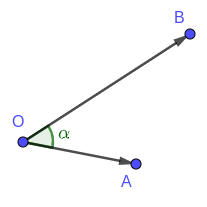
\includegraphics[width=0.4\textwidth]{./cap_produtos/dados/fig_vetangulo/fig_vetangulo}
  \caption{Ângulo entre dois vetores.}
  \label{fig:prodesc_vetangulo}
\end{figure}

\begin{prop}\label{prop:angulo_prodesc}
  Dados $\vec{u}$ e $\vec{v}$, temos
  \begin{equation}\label{eq:prodesc_eq}
    {\color{blue}\vec{u}\cdot\vec{v}=|\vec{u}||\vec{v}|\cos\alpha},
  \end{equation}
  onde $\alpha$ é o ângulo entre os vetores $\vec{u}$ e $\vec{v}$.
\end{prop}
\begin{dem}
  Tomamos as representações $\vec{u} = \overrightarrow{OA}$ e $\vec{v} = \overrightarrow{OB}$. Observamos que $\vec{u}-\vec{v} = \overrightarrow{BA}$. Então, aplicando a lei dos cossenos no triângulo $\triangle OAB$, obtemos
  \begin{equation}
    |\overrightarrow{BA}|^2 = |\overrightarrow{OA}|^2 + |\overrightarrow{OB}|^2 - 2|\overrightarrow{OA}||\overrightarrow{OB}|\cos\alpha,
  \end{equation}
  ou, equivalentemente,
  \begin{align}
    |\vec{u}-\vec{v}|^2 &= |\vec{u}|^2+|\vec{v}|^2-2|\vec{u}||\vec{v}|\cos\alpha\\
    (\vec{u}-\vec{v})\cdot(\vec{u}-\vec{v}) &= |\vec{u}|^2+|\vec{v}|^2-2|\vec{u}||\vec{v}|\cos\alpha\\
    \vec{u}\cdot\vec{u}-2\vec{u}\cdot\vec{v}+\vec{v}\cdot\vec{v} &= |\vec{u}|^2+|\vec{v}|^2-2|\vec{u}||\vec{v}|\cos\alpha\\
    |\vec{u}|^2+|\vec{v}|^2-2\vec{u}\cdot\vec{v} &= |\vec{u}|^2+|\vec{v}|^2-2|\vec{u}||\vec{v}|\cos\alpha
  \end{align}
  donde
  \begin{equation}
    \vec{u}\cdot\vec{v} = |\vec{u}||\vec{v}|\cos\alpha.
  \end{equation}
\end{dem}

\begin{ex}
  Vamos determinar ângulo entre os vetores $\displaystyle \vec{u}=\left(\frac{\sqrt{3}}{2},\frac{1}{2},0\right)$ e $\displaystyle \vec{u}=\left(\frac{1}{2},\frac{\sqrt{3}}{2},0\right)$. Da Proposição \ref{prop:angulo_prodesc}, temos
  \begin{gather}
    {\color{blue}\cos\alpha = \frac{\vec{u}\cdot\vec{v}}{|u|\cdot|v|}}\\
    \cos\alpha = \frac{\frac{\sqrt{3}}{2}\frac{1}{2}+\frac{1}{2}\frac{\sqrt{3}}{2}}{\sqrt{\left(\frac{\sqrt{3}}{2}\right)^2+\left(\frac{1}{2}\right)^2+0^2}\cdot \sqrt{\left(\frac{1}{2}\right)^2+\left(\frac{\sqrt{3}}{2}\right)^2+0^2}}\\
    \cos\alpha = \frac{\frac{\sqrt{3}}{2}}{1\cdot 1} = \frac{\sqrt{3}}{2}.
  \end{gather}
  Portanto, temos $\alpha = \pi/6$.
\end{ex}

\begin{obs}
  O {\bf ângulo} entre dois vetores $\vec{u}$ e $\vec{v}$ é:
  \begin{itemize}
  \item {\bf agudo} se, e somente se, $\vec{u}\cdot\vec{v} > 0$;
  \item {\bf obtuso} se, e somente se, $\vec{u}\cdot\vec{v} < 0$.
  \end{itemize}

  De fato, de \eqref{eq:prodesc_eq}, temos que o sinal de $\vec{u}\cdot\vec{v}$ é igual ao sinal de $\cos\alpha$ (o cosseno do ângulo entre os vetores). Também, por definição, $0 \leq \alpha \leq \pi$. Logo, se $\cos\alpha > 0$, então $0< \alpha < \pi/2$ (ângulo agudo) e, se $\cos\alpha < 0$, então $\pi/2 < \alpha < \pi$ (ângulo obtuso).
\end{obs}

\begin{obs}(Vetores ortogonais) 
  Se $\vec{u},\vec{v}\neq\vec{0}$, então:
  \begin{itemize}
  \item $\vec{u}\perp\vec{v}$ se, e somente se, $\vec{u}\cdot\vec{v}=0$.
  \end{itemize}

  De fato, seja $\alpha$ o ângulo entre $\vec{u}$ e $\vec{v}$. Se $\vec{u}\perp\vec{v}$, então $\alpha = \pi/2$ e
  \begin{align}
    \vec{u}\cdot\vec{v} &= |\vec{u}||\vec{v}|\cos\alpha\\
                        &= |\vec{u}||\vec{v}|\cos\left(\frac{\pi}{2}\right)\\
                        &= |\vec{u}|\cdot |\vec{v}|\cdot 0 \\
                        &= 0.
  \end{align}
  Reciprocamente, se $\vec{u}\cdot\vec{v} = 0$, então
  \begin{align}
    \cos\alpha &= \frac{\vec{u}\cdot\vec{v}}{|\vec{u}||\vec{v}|}\\
               &= \frac{0}{|\vec{u}||\vec{v}|} \\
               &= 0.
  \end{align}
  Lembrando que $0\leq \alpha\leq \pi$, segue que $\alpha = \pi/2$, i.e. $\vec{u}\perp\vec{v}$.
\end{obs}

\begin{ex}
  Os vetores $\vec{i}=(1,0,0)$ e $\vec{u}=(0,1,1)$ são ortogonais. De fato, temos
  \begin{align}
    \vec{i}\cdot\vec{j} &= 1\cdot 0 + 0\cdot 1 + 0\cdot 1 \\
                        &= 0.
  \end{align}
\end{ex}

\subsection{Desigualdade Triangular}

Dados dois vetores $\vec{u}$ e $\vec{v}$ temos
\begin{equation}
  {\color{blue}|\vec{u}+\vec{v}| \leq |\vec{u}| + |\vec{v}|},
\end{equation}
esta é conhecida como a {\bf desigualdade triangular}. Para demonstrá-la, começamos observando que
\begin{align}
  |\vec{u}+\vec{v}|^2 &= (\vec{u}+\vec{v})\cdot(\vec{u}+\vec{v})\\
                      &= \vec{u}\cdot\vec{v}+\vec{v}\cdot\vec{v}+\vec{u}\cdot\vec{v}+\vec{v}\cdot\vec{u}\\
                      &= |\vec{u}|^2 + |\vec{v}|^2 + 2\vec{u}\cdot\vec{v}.  
\end{align}
Agora, vamos estimar $\vec{u}\cdot\vec{v}$. Pela Proposição \ref{prop:angulo_prodesc}, temos
\begin{equation}
  \vec{u}\cdot\vec{v} = |\vec{u}||\vec{v}|\cos\alpha,
\end{equation}
onde $\alpha$ é o ângulo entre $\vec{u}$ e $\vec{v}$. Mas, então:
\begin{equation}
  \vec{u}\cdot\vec{v} \leq |\vec{u}||\vec{v}||\cos\alpha|.
\end{equation}
Daí, como $|\cos\alpha|\leq 1$, temos
\begin{equation}
  {\color{blue}\vec{u}\cdot\vec{v}\leq |\vec{u}||\vec{v}|},
\end{equation}
a qual é chamada de {\bf desigualdade de Cauchy-Schwarz}\footnote{Augustin-Louis Cauchy, 1798-1857, matemático francês. Fonte: \href{https://en.wikipedia.org/wiki/Augustin-Louis_Cauchy}{Wikipeida}. Hermann Schwarz, 1843-1921, matemático alemão. Fonte: \href{https://en.wikipedia.org/wiki/Hermann\_Schwarz}{Wikipedia}.}.

\subsection{Exercícios Resolvidos}

\begin{exeresol}
  Sejam $\vec{u}=(x,-1,2)$ e $\vec{v}=(2,x,-3)$. Determine $x$ tal que
  \begin{equation}
    \vec{u}\cdot\vec{v}=\frac{1}{2}.
  \end{equation}
\end{exeresol}
\begin{resol}
  Da definição do produto escalar, temos
  \begin{gather}
    \vec{u}\cdot\vec{v} = u_1v_1 + u_2v_2 + u_3v_3 \\
    \frac{1}{2} = 2x - x - 6 \\
    x - 6 = \frac{1}{2} \\
    x = \frac{1}{2} + 6 \\
    x = \frac{13}{2}.
  \end{gather}
\end{resol}

\begin{exeresol}
  Determine $x$ tal que $\vec{u}=(-1,0,x)$ seja ortogonal a $\vec{v}=(1,2,-1)$.
\end{exeresol}
\begin{resol}
  Para que $\vec{u}\perp\vec{v}$ devemos ter
  \begin{gather}
    \vec{u}\cdot\vec{v} = 0 \\
    -1 + 0 -x = 0 \\
    x = -1.
  \end{gather}
\end{resol}

\subsection{Exercícios}

\begin{exer}
  Determine o ângulo entre os vetores $\vec{u}=(1,0,1)$ e $\vec{v}=(0,0,2)$.
\end{exer}
\begin{resp}
  $\pi/4$
\end{resp}

\begin{exer}
  Seja $\vec{v} = (1,2,-1)$. Determine a norma do vetor $\vec{u}$ de mesma direção de $\vec{v}$ e tal que $\vec{u}\cdot\vec{v}=2$.
\end{exer}
\begin{resp}
  $\frac{\sqrt{6}}{3}$
\end{resp}

\begin{exer}
  Se $\vec{u}$ e $\vec{v}$ são vetores unitários e $\vec{u}\cdot\vec{v}=1$, então $\vec{u}$ e $\vec{v}$ têm a mesma direção e o mesmo sentido? Justifique sua resposta.
\end{exer}
\begin{resp}
  Sim.
\end{resp}

\begin{exer}
  Se $\vec{u}$ e $\vec{v}$ são vetores tais que $\vec{u}\cdot\vec{v}=-1$, então $\vec{u}$ e $\vec{v}$ têm a mesma direção e sentidos opostos? Justifique sua resposta.
\end{exer}
\begin{resp}
  Não necessariamente.
\end{resp}

\begin{exer}
  Encontre o vetor $x$ ortogonal a $\vec{u}=(1,-2,0)$ e $\vec{v}=(2,-1,1)$ tal que $\vec{x}\cdot(0,-1,2)=1$.
\end{exer}
\begin{resp}
  $\vec{x}=(-2/7,-1/7,3/7)$
\end{resp}

\section{Projeção Ortogonal}\label{cap_produtos_sec_proj}
\badgeRevisar

Sejam dados os vetores $\vec{u}=\overrightarrow{OA}$, $\vec{v}=\overrightarrow{OB}\neq\vec{0}$. Seja, ainda, $P$ a interseção da reta perpendicular a $OB$ que passa pelo ponto $A$. Observemos a Figura \ref{fig:proj}. Com isso, definimos a {\bf projeção ortogonal de $\vec{u}$ na direção de $\vec{v}$}  por $\overrightarrow{OP}$. Denotamos
\begin{equation}
  {\color{blue}\overrightarrow{OP} = \proj_{\vec{v}}\vec{u}}.
\end{equation}

\begin{figure}[H]
  \centering
  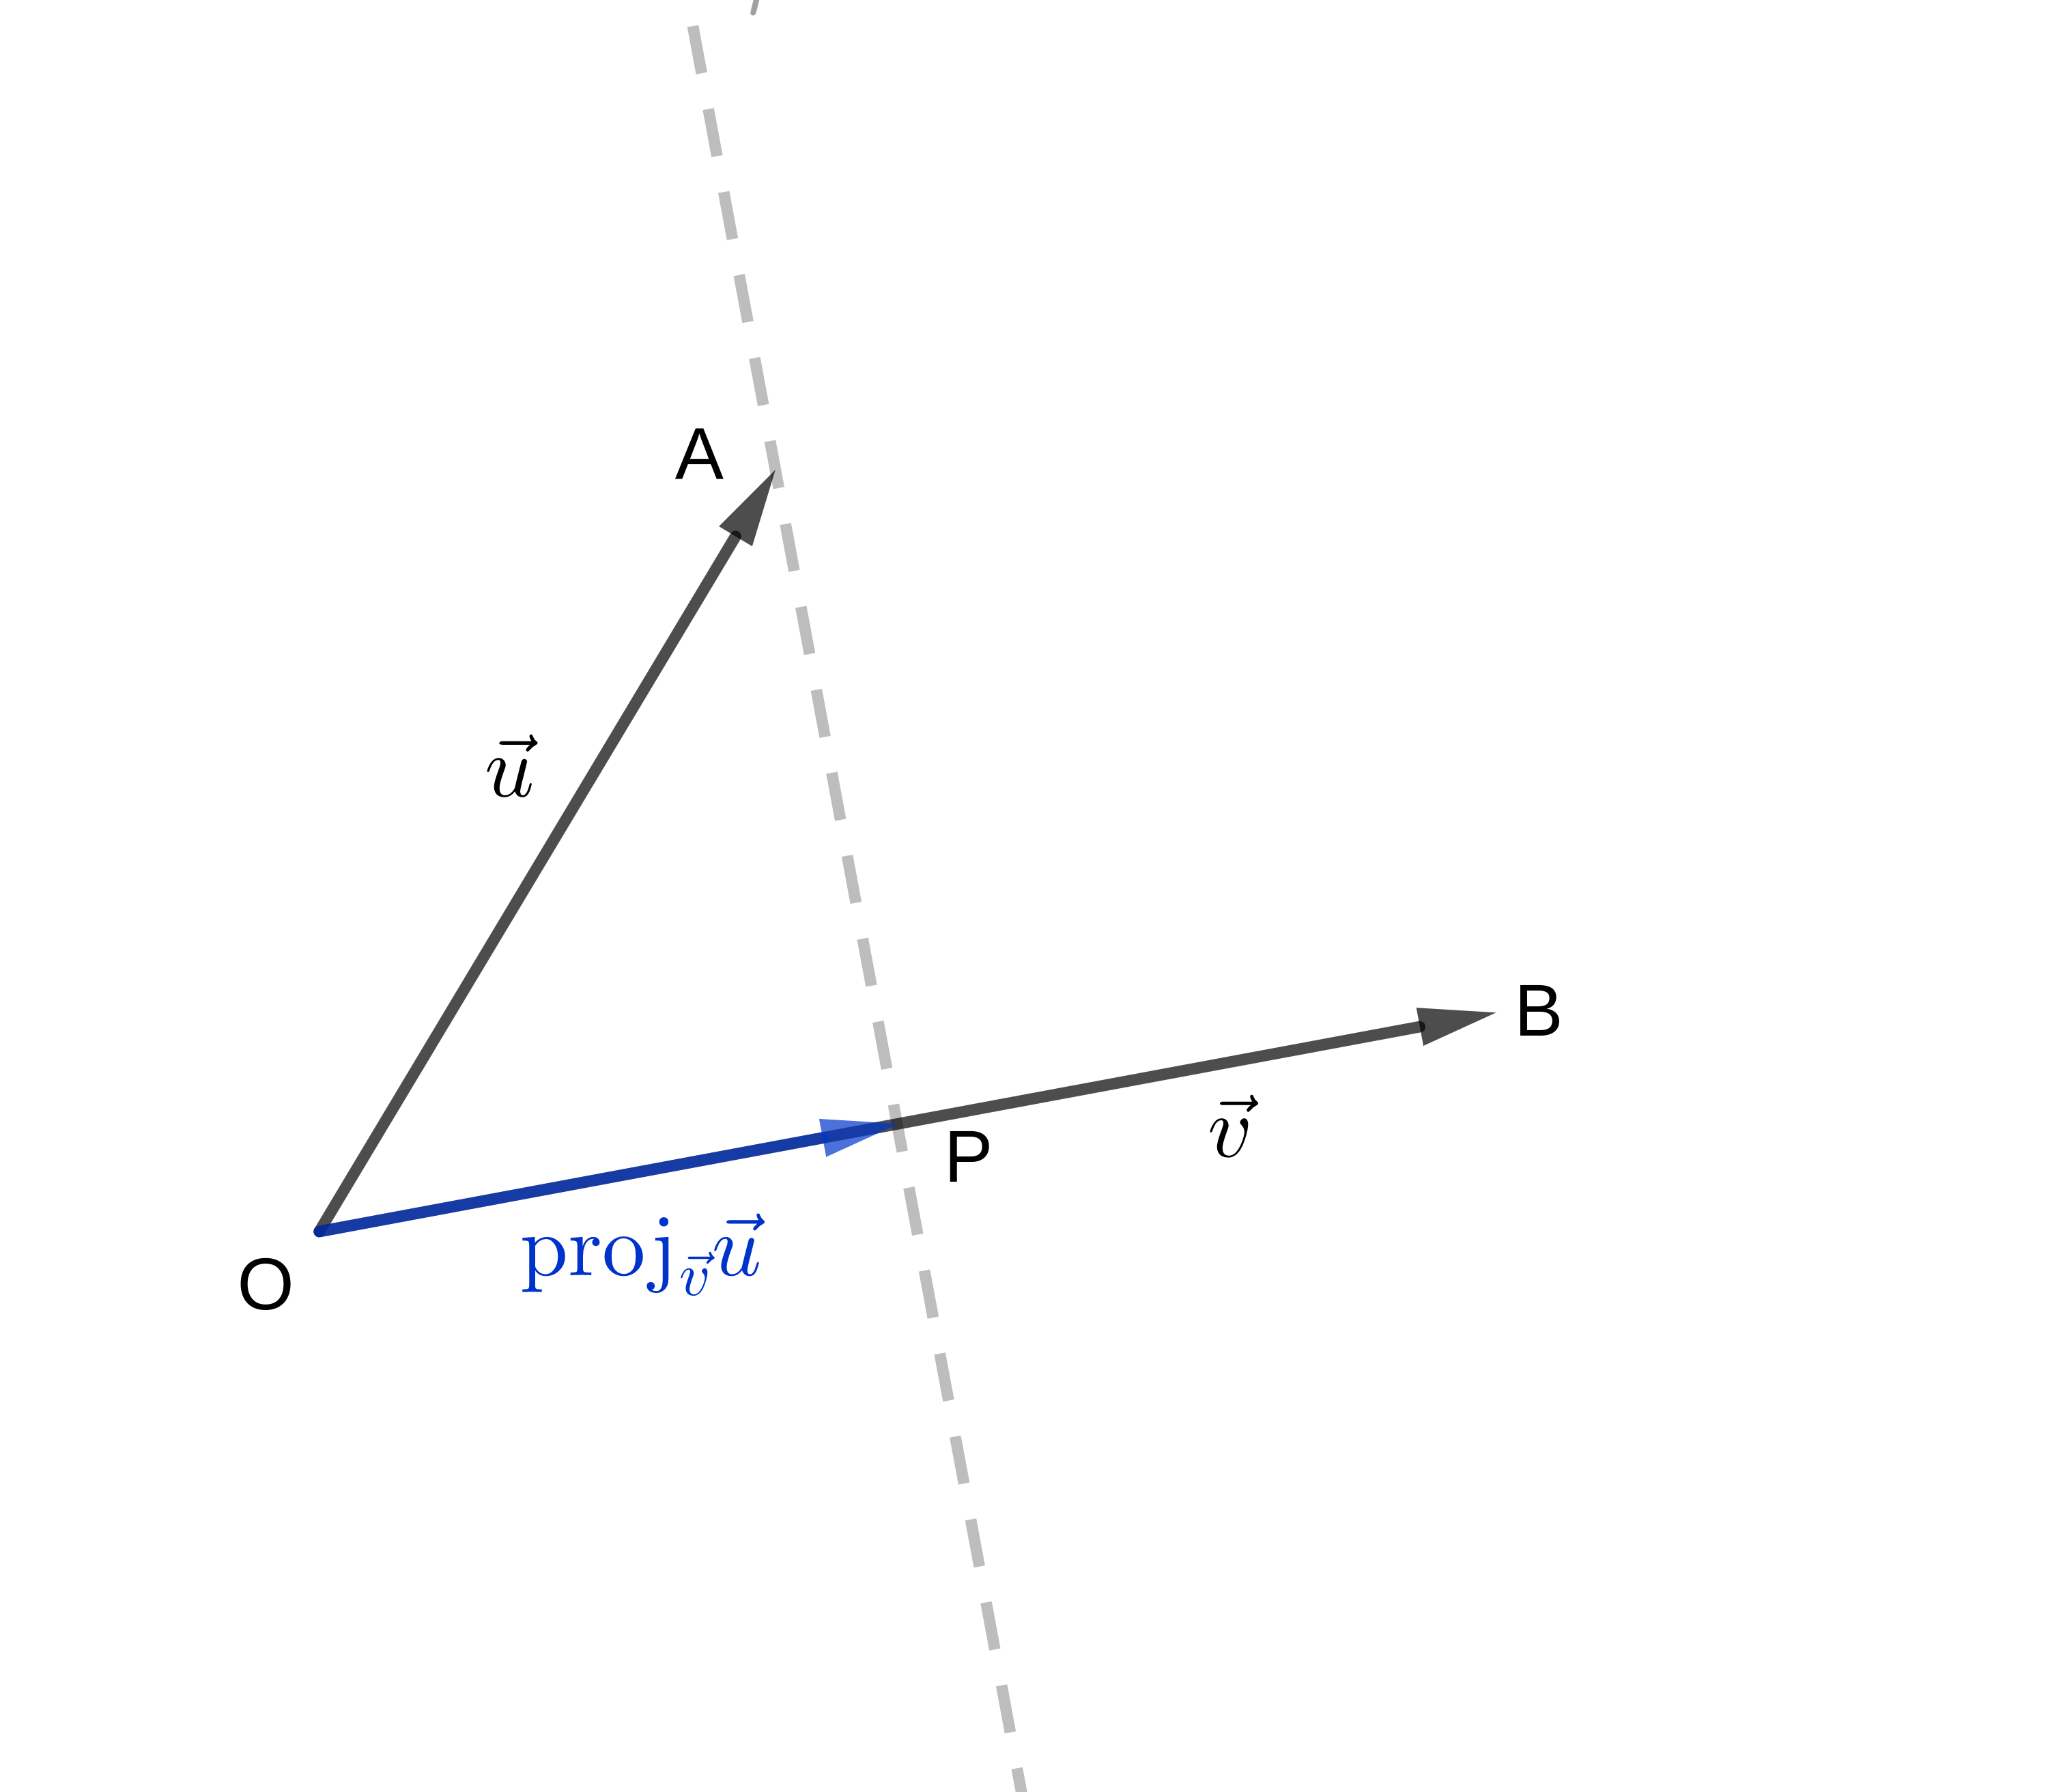
\includegraphics[width=0.7\textwidth]{./cap_produtos/dados/fig_proj/fig_proj}
  \caption{Ilustração da definição da projeção ortogonal.}
  \label{fig:proj}
\end{figure}

Da definição, temos que\footnote{$\proj_{\vec{v}}\vec{u}$ é um vetor múltiplo por escalar de $\vec{v}$.}
\begin{equation}
  {\color{blue}\proj_{\vec{v}}\vec{u} = \beta\cdot \vec{v}}
\end{equation}
para algum número real $\beta$. Além disso, temos
\begin{equation}
  \proj_{\vec{v}}\vec{u} = \vec{u} + \overrightarrow{AP}.
\end{equation}
Portanto
\begin{equation}
  \beta\vec{v} = \vec{u} + \overrightarrow{AP}.
\end{equation}
Tomando o produto escalar com $\vec{v}$ em ambos os lados desta equação, obtemos
\begin{align}
  \beta\vec{v}\cdot\vec{v} &= \vec{u}\cdot\vec{v} + \overrightarrow{AP}\cdot\vec{v} \\
  &= \vec{u}\cdot\vec{v},
\end{align}
pois $\overrightarrow{AP}\perp\vec{v}$. Daí, lembrando que $\vec{v}\cdot\vec{v}=|v|^2$, temos
\begin{equation}
  \alpha = \frac{\vec{u}\cdot\vec{v}}{|\vec{v}|^2}
\end{equation}
e concluímos que
\begin{equation}\label{eq:proj}
  {\color{blue}\proj_{\vec{v}}\vec{u} = \frac{\vec{u}\cdot\vec{v}}{|\vec{v}|^2}\vec{v}}.
\end{equation}

\begin{ex}
  Sejam $\vec{u}=(-1,1,-1)$ e $\vec{v}=(2,1,-2)$. Usando a equação \eqref{eq:proj}, obtemos
  \begin{align}
    \proj_{\vec{v}}\vec{u} &= \frac{(-1,1,-1)\cdot(2,1,-2)}{|(2,1,-2)|^2}(2,1,-2)\\
                           &= \frac{-2+1+2}{4+1+4}(2,1,-2)\\
                           &= \left(\frac{2}{9},\frac{1}{9},\frac{-2}{9}\right).
  \end{align}
\end{ex}

\subsection{Exercícios Resolvidos}

\begin{exeresol}
  Determine $x$ tal que a projeção de $\vec{u}=(1,x,x)$ em $\vec{v}=(1,1,0)$ tenha o dobro da norma de $\vec{v}$.
\end{exeresol}
\begin{resol}
  De \eqref{eq:proj}, a projeção de $\vec{u}$ em $\vec{v}$ é
  \begin{gather}
    \proj_{\vec{v}}\vec{u} = \frac{\vec{u}\cdot\vec{v}}{|\vec{v}|^2}\vec{v},\\
    \left|\proj_{\vec{v}}\vec{u}\right| = \left|\frac{\vec{u}\cdot\vec{v}}{|\vec{v}|^2}\right||\vec{v}| \\
    \left|\proj_{\vec{v}}\vec{u}\right| = \left|\frac{\vec{u}\cdot\vec{v}}{|\vec{v}|}\right| \\
      \left|\proj_{\vec{v}}\vec{u}\right| = \frac{|1+x|}{|\vec{v}|}
  \end{gather}
  Queremos que
  \begin{gather}
    |\proj_{\vec{v}}\vec{u}| = 2|\vec{v}|.
  \end{gather}
  Segue que
  \begin{gather}
    \frac{|1+x|}{|\vec{v}|} = 2|\vec{v}|\\
      |1+x| = 2|\vec{v}|^2 \\
      |1+x| = 2\cdot 2 \\
      1+x = -4\quad\text{ou}\quad 1+x=4\\
      x=-5\quad\text{ou}\quad x=3.
  \end{gather}
\end{resol}

\begin{exeresol}
  Verifique que se $\vec{u}\perp\vec{v}$, então $\proj_{\vec{v}}\vec{u}=\vec{0}$. Justifique sua resposta.
\end{exeresol}
\begin{resol}
  Temos que
  \begin{equation}
    \proj_{\vec{v}}\vec{u} = \frac{\vec{u}\cdot\vec{v}}{|\vec{v}|^2}\vec{v}.
  \end{equation}
  Tendo em vista que $\vec{u}\perp\vec{v}$, temos $\vec{u}\cdot\vec{v}=0$. Logo,
  \begin{align}
    \proj_{\vec{v}}\vec{u} &= 0\cdot\vec{v}\\
                           &= \vec{0}.
  \end{align}
\end{resol}

\subsection{Exercícios}

\begin{exer}
  Sejam $\vec{u}=(-1,1,2)$ e $\vec{v}=(1,-2,0)$. Calcule $\proj_{\vec{v}}\vec{u}$.
\end{exer}
\begin{resp}
  $(-3/5, 6/5, 0)$
\end{resp}

\begin{exer}
  Sejam $\vec{u}$ e $\vec{v}$ vetores unitários e seja $\alpha = \pi/6$ o ângulo entre eles. Calcule a norma da projeção ortogonal de $\vec{u}$ na direção de $\vec{v}$.
\end{exer}
\begin{resp}
  $\frac{\sqrt{3}}{2}$
\end{resp}

\begin{exer}
  Determine $x$ tal que $\proj_{\vec{v}}\vec{u}=(1/6, -1/3, 1/6)$, sendo $\vec{u}=(x,1,2)$ e $\vec{v}=(1,-2,1)$.
\end{exer}
\begin{resp}
  $1$
\end{resp}

\begin{exer}
  Verifique se a $\proj_{\vec{v}}\vec{u}$ tem o mesmo sentido de $\vec{v}$ para quaisquer vetores $\vec{u}$ e $\vec{v}$ dados. Justifique sua resposta.
\end{exer}
\begin{resp}
  Falso
\end{resp}

\begin{exer}
  Determine as coordenadas de todos os vetores $\vec{u}$ tais que $\proj_{\vec{v}}\vec{u}=\vec{v}$, sendo que $\vec{v}=(1,0,0)$.
\end{exer}
\begin{resp}
  $(1,u_2,u_3),~u_1,u_2\in\mathbb{R}$
\end{resp}

\section{Produto Vetorial}\label{cap_produtos_sec_cross}
\badgeRevisar

De agora em diante, vamos trabalhar com um base ortonormal $B = (\vec{i}, \vec{j}, \vec{k})$ dita com \emph{orientação positiva}, i.e. os vetores $\vec{i} = \overrightarrow{OI}$, $\vec{j} = \overrightarrow{OJ}$ e $\vec{k}=\overrightarrow{OK}$ estão dispostos em sentido anti-horário, veja Figura \ref{cap_produtos_sec_cross:fig:base_pos}.

\begin{figure}[H]
  \centering
  \includegraphics[width=0.7\textwidth]{./cap_prodvet/dados/fig_base_pos/fig_base_pos}
  \caption{Base ortonormal com orientação positiva.}
  \label{cap_produtos_sec_cross:fig:base_pos}
\end{figure}

Dados vetores $\vec{u}$ e $\vec{v}$, definimos o produto vetorial de $\vec{u}$ com $\vec{v}$, por
\begin{equation}\label{cap_produtos_sec_cross:eq:def_cross}\hleq
  \vec{u}\cross\vec{v} = \|\vec{u}\|\|\vec{v}\|\sen(\alpha)\vec{n},
\end{equation}
onde $\theta$ é ângulo entre $\vec{u}$ e $\vec{v}$, e $\vec{n}$ é o vetor unitário ortogonal ao plano determinado por $\vec{u}$ e $\vec{v}$, e com sentido tal que $(\vec{u}, \vec{v}, \vec{n})$ tem orientação positiva.

Em outras palavras, temos que:
\begin{itemize}
\item se $\vec{u}$ e $\vec{v}$ são l.d., então $\vec{u}\cross\vec{v} = \vec{0}$.
\item se $\vec{u}$ e $\vec{v}$ são l.i., então
  \begin{itemize}
  \item[a)] $\|\vec{u}\cross\vec{v}\| = \|\vec{u}\|\|\vec{v}\|\sen\alpha$, onde $\alpha$ é o ângulo entre $\vec{u}$ e $\vec{v}$,
  \item[b)] $\vec{u}\cross\vec{v}$ é ortogonal a $\vec{u}$ e $\vec{v}$, e
  \item[c)] $\vec{u}$, $\vec{v}$ e $\vec{u}\cross\vec{v}$ formam uma base positiva.
  \end{itemize}
\end{itemize}

\subsection{Interpretação Geométrica}

Sejam dados $\vec{u}$ e $\vec{v}$ l.i.. Estes vetores determinam um paralelogramo (consulte Figura~\ref{fig:prodvet_interp} (esquerda)). Seja, então, $h$ a altura deste paralelogramo tendo $\vec{u}$ como sua base. Logo, a área do paralelogramo é o produto do comprimento da base com sua altura, neste caso
\begin{align}
  \|\vec{u}\|h &= \|\vec{u}\|\|\vec{v}\|\sen(\alpha)\\
               &= \|\vec{u}\cross\vec{v}\|.
\end{align}
Ou seja, o produto vetorial $\vec{u}\cross\vec{v}$ tem norma igual à área do paralelogramo determinado por $\vec{u}$ e $\vec{v}$.

Ainda, por definição, $\vec{u}\cross\vec{v}$ é ortogonal a $\vec{u}$ e $\vec{v}$. Isto nos dá a direção de $\vec{u}\cross\vec{v}$. O sentido é, então, determinado pela definição de que $(\vec{u},\vec{v},\vec{u}\cross\vec{v})$ tem orientação positiva. Consulte a Figura \ref{fig:prodvet_interp} (direita).

\begin{figure}[H]
  \centering
  \includegraphics[width=0.7\textwidth]{./cap_prodvet/dados/fig_prodvet_interp/fig_prodvet_interp}
  \caption{Interpretação geométrica do produto vetorial.}
  \label{fig:prodvet_interp}
\end{figure}

\subsection{Vetores Canônicos}

Vamos ver alguns resultados fundamentais envolvendo o \hl{produto vetorial de vetores da base canônica}.

\begin{itemize}
  \item $\hleq\vec{i}\cross\vec{i}=\vec{j}\cross\vec{j}=\vec{k}\cross\vec{k}=\vec{0}$
  
  Segue, imediatamente, da definição de que é nulo o produto vetorial de vetores l.i..

  \item $\hleq\vec{i}\cross\vec{j}=\vec{k}$, ~$\hleq\vec{j}\cross\vec{k}=\vec{i}$, ~$\hleq\vec{k}\cross\vec{i}=\vec{j}$
  
  No primeiro caso, temos
  \begin{align}
    \vec{i}\times\vec{j} &:= \|\vec{i}\|\|\vec{j}\|\sen(\alpha)\vec{n}\\
    &= 1\cdot 1\cdot\sen\left(\frac{\pi}{2}\right)\vec{k}\\
    &= \vec{k}.
  \end{align}
  Análogo para os outros casos. Consulte o \exerref{cap_produtos_sec_cross:exer:ijk}.

  \item $\hleq\vec{j}\cross\vec{i}=-\vec{k}$, ~$\hleq\vec{k}\cross\vec{j}=-\vec{i}$, ~$\hleq\vec{i}\cross\vec{k}=-\vec{j}$
  
  No primeiro, temos
  \begin{align}
    \vec{j}\times\vec{i} &:= \|\vec{j}\|\|\vec{i}\|\sen(\theta)\vec{n}\\
    &= 1\cdot 1\cdot\sen\left(\frac{\pi}{2}\right)(-\vec{k})\\
    &= -\vec{k}.
  \end{align}
  Análogo para os outros casos. Consulte o \exerref{cap_produtos_sec_cross:exer:jki}.
\end{itemize}

\subsubsection{Distributividade}

A propriedade de distributividade do produto vetorial com vetores da base canônica também pode ser mostrada. Por exemplo, é verdade que
\begin{equation}\label{cap_produtos_sec_cross:eq:distijk}
  \vec{i}\cross(\vec{j}+\vec{k}) = \vec{i}\cross\vec{j}+\vec{i}\cross\vec{k}.
\end{equation}
De fato, assumindo $\vec{n}$ o vetor normal unitário aos vetores $\vec{i}$ e $\vec{j}+\vec{k}$, temos
\begin{align}
  \vec{i}\cross(\vec{j}+\vec{k}) &:= \|\vec{i}\|\|\vec{j}+\vec{k}\|\sen\left(\frac{\pi}{2}\right)\vec{n}\\
                                 &= 1\cdot \sqrt{2}\cdot 1\vec{n} = \sqrt{2}\vec{n}.\label{cap_produtos_sec_cross:eq:distaux}
\end{align}
Por outro lado, temos
\begin{align}
  \vec{i}\cross\vec{j} + \vec{i}\cross\vec{k} = \vec{k} - \vec{j}
\end{align}
Seria, então,
\begin{equation}
  \vec{n} \stackrel{?}{=} \frac{\sqrt{2}}{2}\vec{k} - \frac{\sqrt{2}}{2}\vec{j}
\end{equation}
De fato, enquanto a positividade de $(\vec{i}, \vec{j}+\vec{k}, \vec{n})$ e a norma unitária $\|\vec{n}\|=1$ são diretas, a ortogonalidade pode ser mostrada do produto interno
\begin{align}
  \vec{i}\cdot\vec{n} &= \vec{i}\cdot\left(\frac{\sqrt{2}}{2}\vec{k} - \frac{\sqrt{2}}{2}\vec{j}\right)\\
  &= \frac{\sqrt{2}}{2}\vec{i}\cdot\vec{k} - \frac{\sqrt{2}}{2}\vec{i}\cdot\vec{j}\\
  &= 0 + 0 = 0
\end{align}
o que mostra que $\vec{i}\perp\vec{n}$. Bem como, temos
\begin{align}
  \left(\vec{j}+\vec{k}\right)\cdot\vec{n} &= \left(\vec{j}+\vec{k}\right)\cdot\left(\frac{\sqrt{2}}{2}\vec{k} - \frac{\sqrt{2}}{2}\vec{j}\right)\\
  &= \frac{\sqrt{2}}{2}\left(\vec{j}\cdot\vec{k}-\vec{j}\cdot\vec{j}+\vec{k}\cdot\vec{k}-\vec{k}\cdot\vec{j}\right)\\
  &= \frac{\sqrt{2}}{2}(0-1+1-0) = 0,
\end{align}
donde concluímos que $(\vec{j}+\vec{k})\perp\vec{n}$. Isso mostra que
\begin{equation}
  \vec{n} = \frac{\sqrt{2}}{2}\vec{k} - \frac{\sqrt{2}}{2}\vec{j}
\end{equation}
e, portanto, de \eqref{cap_produtos_sec_cross:eq:distaux}
\begin{align}
  \vec{i}\cross(\vec{j}+\vec{k}) &= \sqrt{2}\vec{n}\\
  &= \sqrt{2}\left(\frac{\sqrt{2}}{2}\vec{k} - \frac{\sqrt{2}}{2}\vec{j}\right)\\
  &= \vec{k} - \vec{j}\\
  &= \vec{i}\cross\vec{j} + \vec{i}\cross\vec{k}.
\end{align}

\begin{proposicao}\normalfont{(\hl{Distributividade para Vetores Canônicos}.)}
  Se $\vec{u}$, $\vec{v}$ e $\vec{w}$ são vetores da base canônica\footnote{$\vec{i}$, $\vec{j}$ ou $\vec{k}$.}, então vale a distributividade do produto vetorial
  \begin{equation}
    \vec{u}\cross(\vec{v}+\vec{w}) = \vec{u}\cross\vec{v}+\vec{u}\cross\vec{w}.
  \end{equation}
\end{proposicao}
\begin{demonstracao}
  Consulte o \exerref{cap_produtos_sec_cross:exer:distcanonicos}.
\end{demonstracao}

\subsection{Associatividade por Escalar}

Uma das propriedades fundamentais do produto vetorial é a \hl{associatividade com a multiplicação por escalar}
\begin{equation}\label{cap_produtos_sec_cross:eq:associatividade_por_escalar}
  \hleq(\alpha\vec{u})\cross\vec{v} = \alpha \vec{u}\cross\vec{v}.
\end{equation}

Para mostrarmos isso, vamos precisar do seguinte resultado.

\subsubsection{Mudança do Sentido}\label{cap_produtos_sec_cross:sssec:mudanca_de_sentido}

No produto vetores $\vec{u}\cross \vec{v}$, ao mudarmos o sentido de apenas um dos vetores, obtemos a seguinte relação
\begin{equation}\label{cap_produtos_sec_cross:eq:mudanca_do_sentido}
  \hleq(-\vec{u})\times\vec{v} = -(\vec{u}\times\vec{v}) = \vec{u}\times(-\vec{v}).
\end{equation}
De fato, assumindo que o ângulo $\theta$ e o vetor unitário $\vec{n}$ são tais que
\begin{equation}
  \vec{u}\cross\vec{v} = \|\vec{u}\|\|\vec{v}\|\sen(\theta)\vec{n},
\end{equation}
temos
\begin{align}
  (-\vec{u})\cross\vec{v} &= \|-\vec{u}\|\|\vec{v}\|\sen(\theta)(-\vec{n})\\
  &= |-1|\|\vec{u}\|\|\vec{v}\|\sen(\theta)(-\vec{n})\\
  &= -\|\vec{u}\|\|\vec{v}\|\sen(\theta)\vec{n}.
\end{align}
E, de forma análoga, segue que $\vec{u}\cross(-\vec{v}) = -\vec{u}\cross\vec{v}$ (consulte o \exerref{cap_produtos_sec_cross:exer:mudanca_de_sentido}).

\subsubsection{Associatividade com Multiplicação por Escalar}\label{cap_produtos_sec_cross:sssec:associatividade_por_escalar}

Agora, temos tudo para mostrar a associatividade
\begin{equation}
  (\alpha\vec{u})\cross\vec{v} = \alpha(\vec{u}\cross\vec{v}).
\end{equation}
De fato, assumindo $\alpha>0$, o ângulo $\theta$ e o vetor normal unitário $\vec{n}$ tais que
\begin{equation}
  \vec{u}\cross\vec{v} = \|\vec{u}\|\|\vec{v}\|\sen(\theta)\vec{n},
\end{equation}
temos que\footnote{Observamos que $\protect\vec{u}$ também é vetor normal unitário aos vetores $\protect\alpha\vec{u}$ e $\protect\vec{v}$.}
\begin{align}
  (\alpha\vec{u})\cross\vec{v} &= \|\alpha \vec{u}\|\|\vec{v}\|\sen(\theta)\vec{n}\\
  &= |\alpha|\|\vec{u}\|\|\vec{v}\|\sen(\theta)\vec{n}\\
  &= \alpha\|\vec{u}\|\|\vec{v}\|\sen(\theta)\vec{n}\\
  &= \alpha(\vec{u}\cross\vec{v}).
\end{align}
No caso de $\alpha < 0$, o resultado da propriedade da mudança do sentido \eqref{cap_produtos_sec_cross:eq:mudanca_do_sentido}, i.e.
\begin{align}
  (\alpha\vec{u})\cross\vec{v} &= -(-\alpha\vec{u})\cross\vec{v}\\
  &= -(-\alpha)(\vec{u}\cross\vec{v})\\
  &= \alpha(\vec{u}\cross\vec{v}).
\end{align}
Por raciocínio análogo, segue também que
\begin{equation}
  \vec{u}\cross(\alpha\vec{v}) = \alpha(\vec{u}\cross\vec{v})
\end{equation}
para qualquer escalar $\alpha$ (consulte o \exerref{cap_produtos_sec_cross:exer:associatividade_por_escalar}).


\subsection{Produto Vetorial por Coordenadas}\label{cap_prodvet_sec_coord}

Usando as propriedades que estudamos até aqui, vamos mostrar que dados $\vec{u} = (u_1,u_2,u_3)$ e $\vec{v} = (v_1,v_2,v_3)$ em uma base ortonormal positiva, então
\begin{equation}
  \vec{u}\cross\vec{v} =
  \begin{vmatrix}
    u_2 & u_3\\
    v_2 & v_3
  \end{vmatrix}\vec{i} -
  \begin{vmatrix}
    u_1 & u_3\\
    v_1 & v_3
  \end{vmatrix}\vec{j} +
  \begin{vmatrix}
    u_1 & u_2 \\
    v_1 & v_2
  \end{vmatrix}\vec{k}
\end{equation}
ou, mnemonicamente,
\begin{equation}\label{cap_produtos_sec_cross:eq:cross_coords}\hleq
  \vec{u}\cross\vec{v} =
  \begin{vmatrix}
    \vec{i} & \vec{j} & \vec{k} \\
    u_1 & u_2 & u_3 \\
    v_1 & v_2 & v_3
  \end{vmatrix}.
\end{equation}
De fato, das propriedades da distributividade e da associatividade estudadas, temos
\begin{align}
  \vec{u}\times\vec{v} &= (u_1\vec{i}+u_2\vec{j}+u_3\vec{k})\\
  &\quad \cross(v_1\vec{i}+v_2\vec{j}+v_3\vec{k})\\
  &= (u_2v_3-u_3v_2)\vec{i}\\
  &\quad + (u_3v_1-u_1v_3)\vec{j}\\
  &\quad + (u_1v_2-u_2v_1)\vec{k}\\
  &= \begin{vmatrix}
    u_2 & u_3\\
    v_2 & v_3
  \end{vmatrix}\vec{i}\\
  &\quad -
  \begin{vmatrix}
    u_1 & u_3\\
    v_1 & v_3
  \end{vmatrix}\vec{j}\\
  &\quad +
  \begin{vmatrix}
    u_1 & u_2 \\
    v_1 & v_2
  \end{vmatrix}\vec{k}.
\end{align}
Temos, portanto, mostrado \eqref{cap_produtos_sec_cross:eq:cross_coords}.

\begin{ex}
  Dados os vetores $\vec{u} = (1,-2,1)$ e $\vec{v} = (0,2,-1)$, temos
  \begin{align}
    \vec{u}\cross\vec{v} &=
                          \begin{vmatrix}
                            \vec{i} & \vec{j} & \vec{k} \\
                            u_1 & u_2 & u_3 \\
                            v_1 & v_2 & v_3
                          \end{vmatrix} \\
                        &=
                          \begin{vmatrix}
                            \vec{i} & \vec{j} & \vec{k} \\
                            1       & -2      & 1 \\
                            0       & 2       & -1
                          \end{vmatrix} \\
                        &= 0\vec{i} + \vec{j} + 2\vec{k}\\
                        &= (0,1,2).
  \end{align}
\end{ex}

\subsection{Exercícios Resolvidos}

\begin{exeresol}
  Calcule $\vec{x}$ tal que $(0,2,-1)\cross\vec{x}=(-3,-1,-2)$.
\end{exeresol}
\begin{resol}
  Denotando $\vec{x}=(x_1,x_2,x_3)$, temos
  \begin{gather}
    (0,2,-1)\cross\vec{x}=(-3,-1,-2)\\
    \begin{vmatrix}
      \vec{i} & \vec{j} & \vec{k} \\
      0 & 2 & -1 \\
      x_1 & x_2 & x_3
    \end{vmatrix} = (-3,-1,-2)\\
    (x_2+2x_3)\vec{i}-x_1\vec{j}-2x_1\vec{k} = \\
    -3\vec{i}-\vec{j}-2\vec{k}
  \end{gather}
  Segue que
  \begin{align*}
    x_2+2x_3 &= -3\\
    -x_1 &= -1\\
    -2x_1 &= -2
  \end{align*}
  Logo, $x_1 = 1$, $x_2=-3-2x_3$ e $x_3$ é arbitrário. Concluímos que $\vec{x} = (1,-3-2x_3,x_3)$ com $x_3\in\mathbb{R}$.
\end{resol}

\begin{exeresol}
  Determine a área do paralelogramo determinado pelos vetores $\vec{u} = (-1, 2, 3)$ e $\vec{v} = (1,-2,1)$.
\end{exeresol}
\begin{resol}
  Tomando representações $\vec{u}=\overrightarrow{OA}$ e $\vec{v}=\overrightarrow{OC}$, temos que $\vec{u}$ e $\vec{v}$ determinam um paralelogramo $OABC$, onde $B$ é tal que $\vec{u}+\vec{v}=\overrightarrow{OB}$\footnote{Consulte a regra do paralelogramo na Subseção~\ref{cap_vetor_sec_op:sssec:regra_do_paralelogramo}.}. Da definição do produto vetorial, temos que
  \begin{equation}
    \|\vec{u}\cross\vec{v}\| = \|\vec{u}\|\|\vec{v}\|\sen\theta,
  \end{equation}
  o que é igual a área do paralelogramo $OABC$, onde $\theta$ é o ângulo entre os vetores $\vec{u}$ e $\vec{v}$. Logo, a área do paralelogramo é
  \begin{gather}
    \|\vec{u}\cross\vec{v}\| =
    \left|\begin{vmatrix}
      \vec{i} & \vec{j} & \vec{k} \\
      -1 & 2 & 3 \\
      1 & -2 & 1
    \end{vmatrix}\right|\\
    \|\vec{u}\cross\vec{v}\| = \|(8,4,0)\|\\
    \|\vec{u}\cross\vec{v}\| = 4\sqrt{5}.
  \end{gather}
\end{resol}

\subsection{Exercícios}

\begin{exer}\label{cap_produtos_sec_cross:exer:ijk}
  A partir da definição do produto vetorial \eqref{cap_produtos_sec_cross:eq:def_cross}, calcule
  \begin{enumerate}[a)]
    % a)
    \item $\vec{i}\times\vec{j}$
    % b)
    \item $\vec{j}\times\vec{k}$
    % c)
    \item $\vec{k}\times\vec{i}$
  \end{enumerate}
\end{exer}
\begin{resp}
  a) $\vec{k}$; b) $\vec{i}$; c) $\vec{j}$
\end{resp}

\begin{exer}
  Repita o \exerref{cap_produtos_sec_cross:exer:ijk}, calculando cada item a partir do cálculo do produto vetorial por coordenadas \eqref{cap_produtos_sec_cross:eq:cross_coords}.
\end{exer}
\begin{resp}
  a) $\vec{k}$; b) $\vec{i}$; c) $\vec{j}$
\end{resp}


\begin{exer}\label{cap_produtos_sec_cross:exer:jki}
  A partir da definição do produto vetorial \eqref{cap_produtos_sec_cross:eq:def_cross}, calcule
  \begin{enumerate}[a)]
    % a)
    \item $\vec{j}\times\vec{i}$
    % b)
    \item $\vec{k}\times\vec{j}$
    % c)
    \item $\vec{i}\times\vec{k}$
  \end{enumerate}
\end{exer}
\begin{resp}
  a) $-\vec{k}$; b) $-\vec{i}$; c) $-\vec{j}$
\end{resp}

\begin{exer}
  Repita o \exerref{cap_produtos_sec_cross:exer:jki}, calculando cada item a partir do cálculo do produto vetorial por coordenadas \eqref{cap_produtos_sec_cross:eq:cross_coords}.
\end{exer}
\begin{resp}
  a) $-\vec{k}$; b) $-\vec{i}$; c) $-\vec{j}$
\end{resp}

\begin{exer}\label{cap_produtos_sec_cross:exer:distcanonicos}
  A partir da definição do produto vetorial \eqref{cap_produtos_sec_cross:eq:def_cross}, mostre que
  \begin{enumerate}[a)]
    \item $\vec{i}\cross(\vec{i}+\vec{j}) = \vec{k}$
    \item $\vec{j}\cross(\vec{j}+\vec{k}) = \vec{i}$
    \item $\vec{j}\cross(\vec{i}+\vec{k}) = -\vec{k}+\vec{i}$
    \item $\vec{k}\cross(\vec{i}+\vec{j}) = \vec{j}-\vec{i}$
    \item $\vec{k}\cross(\vec{i}+\vec{k}) = \vec{j}$
    \item $\vec{k}\cross(\vec{j}+\vec{k}) = -\vec{i}$
  \end{enumerate}
\end{exer}
\begin{resp}
  Dica: consulte a demonstração da \eqref{cap_produtos_sec_cross:eq:distijk}.
\end{resp}

\begin{exer}
  Sejam $\vec{u}=(2,-3,1)$ e $\vec{v}=(1,-2,-1)$. Calcule:
  \begin{enumerate}[a)]
  \item $\vec{u}\cross\vec{v}$.
  \item $\vec{v}\cross\vec{u}$.
  \item $\vec{v}\cross(2\vec{u})$.
  \end{enumerate}
\end{exer}
\begin{resp}
  a)~$(5,3,-1)$; b)~$(-5,-3,1)$; c)~$(-10,-6,2)$
\end{resp}

\begin{exer}
  Sejam $\vec{u}$ e $\vec{v}$ tais que $\vec{u}\cross\vec{v}=(2,-1,0)$. Forneça $\vec{v}\cross\vec{u}$. Justifique sua resposta.
\end{exer}
\begin{resp}
  $(-2,1,0)$
\end{resp}

\begin{exer}
  Seja $\vec{u}$ um vetor qualquer. Calcule $\vec{u}\cross\vec{u}$.
\end{exer}
\begin{resp}
  $0$
\end{resp}

\begin{exer}
  Sejam $\vec{u}$ e $\vec{v}$ tais que $(2\vec{u})\cross\vec{v}=(2,-1,0)$. Forneça $\vec{v}\cross\vec{u}$. Justifique sua resposta.
\end{exer}
\begin{resp}
  $(-1,1/2,0)$
\end{resp}

\begin{exer}
  Calcule $\vec{x}$ tal que $\vec{x}\cross (2,-2,3)=(11,8,-2)$.
\end{exer}
\begin{resp}
  $\left(\frac{2}{3}x_3-\frac{8}{3},-\frac{2}{3}x_3+\frac{11}{3},x_3\right), x_3\in\mathbb{R}$
\end{resp}

\begin{exer}\label{cap_produtos_sec_cross:exer:mudanca_de_sentido}
  A partir da definição de produto vetorial \eqref{cap_produtos_sec_cross:eq:def_cross}, mostre que
  \begin{equation}
    \vec{u}\times(-\vec{v}) = -\vec{u}\times\vec{v}.
  \end{equation}
\end{exer}
\begin{resp}
  Dica: estude a Subseção~\ref{cap_produtos_sec_cross:sssec:mudanca_de_sentido}.
\end{resp}

\begin{exer}\label{cap_produtos_sec_cross:exer:associatividade_por_escalar}
  Mostre que vale a seguinte associatividade com multiplicação por escalar
  \begin{equation}
    \vec{u}\cross(\alpha\vec{v}) = \alpha(\vec{u}\cross\vec{v}),
  \end{equation}
  para quaisquer vetores $\vec{u}$, $\vec{v}$ e escalar $\alpha$.
\end{exer}
\begin{resp}
  Dica: estude a Subseção~\ref{cap_produtos_sec_cross:sssec:associatividade_por_escalar}.
\end{resp}


\section{Propriedades do Produto Vetorial}\label{cap_prodvet_sec_prop}
\badgeRevisar

Nesta seção, discutiremos sobre algumas propriedades do produto vetorial. Para tanto, sejam dados os vetores $\vec{u} = (u_1,u_2,u_3)$, $\vec{v}=(v_1,v_2,v_3)$, $\vec{w}=(w_1,w_2,w_3)$ e o número real $\gamma$.

Da definição do produto vetorial, temos $\vec{u}\perp(\vec{u}\cross\vec{v})$ e $\vec{v}\perp(\vec{u}\cross\vec{v})$, logo
\begin{equation}
  {\color{blue}\vec{u}\cdot(\vec{u}\cross\vec{v}) = 0}
\end{equation}
e
\begin{equation}
  {\color{blue}\vec{v}\cdot(\vec{u}\cross\vec{v}) = 0}.
\end{equation}

\begin{ex}
  Sejam $\vec{u}=(1,-1,2)$, $\vec{v}=(2,-1,-2)$. Temos
  \begin{align}
    \vec{u}\cross\vec{v} &=
    \begin{vmatrix}
      \vec{i} & \vec{j} & \vec{k} \\
      1 & -1 & 2 \\
      2 & -1 & -2
    \end{vmatrix}\\
              &= (4,6,1)
  \end{align}
  Segue, que
  \begin{align}
    \vec{u}\cdot(\vec{u}\cross\vec{v}) &= (1,-1,2)\cdot (4,6,1) \\
                                      &= 4-6+2\\
                                      &= 0.
  \end{align}
\end{ex}

Em relação à multiplicação por escalar, temos
\begin{align}
  {\color{blue}\gamma(\vec{u}\cross\vec{v})} &= {\color{red}(\gamma\vec{u})\cross\vec{v}} \\
                              &= {\color{cyan}\vec{u}\cross(\gamma\vec{v})}.
\end{align}
De fato,
\begin{align}
  {\color{red}(\gamma\vec{u})\cross\vec{v}} &=
                                {\color{red}\begin{vmatrix}
                                  \vec{i} & \vec{j} & \vec{k} \\
                                  \gamma u_1 & \gamma u_2 & \gamma u_3\\
                                  v_1 & v_2 & v_3
                                \end{vmatrix}} \\
                              &= {\color{blue}\gamma\begin{vmatrix}
                                  \vec{i} & \vec{j} & \vec{k} \\
                                  u_1 & u_2 & u_3\\
                                  v_1 & v_2 & v_3
                                \end{vmatrix}} = {\color{blue}\gamma(\vec{u}\cross\vec{v})}\\
                              &=
                                {\color{cyan}\begin{vmatrix}
                                  \vec{i} & \vec{j} & \vec{k} \\
                                  u_1 & u_2 & u_3\\
                                  \gamma v_1 & \gamma v_2 & \gamma v_3
                                \end{vmatrix}} = {\color{cyan}\vec{u}\cross(\gamma\vec{v})}
\end{align}

\begin{ex}
  Sejam $\vec{u}=(1,-1,2)$ e $\vec{v}=(2,-1,-2)$. Temos
  \begin{align}
    {\color{blue}2(\vec{u}\cross\vec{v})} &=
    2\begin{vmatrix}
      \vec{i} & \vec{j} & \vec{k} \\
      1 & -1 & 2 \\
      2 & -1 & -2
    \end{vmatrix}\\
                           &= 2(4,6,1)\\
                           &= (8,12,2)
  \end{align}
  \begin{align}
    {\color{red}(2\vec{u})\cross\vec{v}} &=
    \begin{vmatrix}
      \vec{i} & \vec{j} & \vec{k} \\
      2 & -2 & 4 \\
      2 & -1 & -2
    \end{vmatrix}\\
                           &= (8,12,2)
  \end{align}
  \begin{align}
    {\color{cyan}\vec{u}\cross(2\vec{v})} &=
    \begin{vmatrix}
      \vec{i} & \vec{j} & \vec{k} \\
      1 & -1 & 2 \\
      4 & -2 & -4
    \end{vmatrix}\\
                           &= (8,12,2)
  \end{align}
\end{ex}


Também, vale a {\color{blue}propriedade distributiva com a operação de soma}, i.e.
\begin{equation}
  {\color{blue}\vec{u}\cross(\vec{v} + \vec{w}) = \vec{u}\cross\vec{v}+\vec{u}\cross\vec{w}}.
\end{equation}
De fato, temos
\begin{gather}
  \vec{u}\cross(\vec{v}+\vec{w}) \\
  = \begin{vmatrix}
    \vec{i} & \vec{j} & \vec{k} \\
    u_1 & u_2 & u_3 \\
    v_1+w_1 & v_2+w_2 & u_3+w_3
  \end{vmatrix} \\
  = \begin{vmatrix}
    \vec{i} & \vec{j} & \vec{k} \\
    u_1 & u_2 & u_3 \\
    v_1 & v_2 & v_3
  \end{vmatrix}
  +  \begin{vmatrix}
    \vec{i} & \vec{j} & \vec{k} \\
    u_1 & u_2 & u_3 \\
    w_1 & w_2 & w_3
  \end{vmatrix}\\
  = \vec{u}\cross\vec{v} + \vec{u}\cross\vec{w}.
\end{gather}

\begin{ex}
  Sejam $\vec{u}=(1,-1,2)$, $\vec{v}=(2,-1,-2)$ e $\vec{w}=(0,-1,-1)$. Temos
  \begin{gather}
    \vec{u}\cross(\vec{v}+\vec{w}) \\
    = \vec{u}\cross \left[(2,-1,-2)+(0,-1,-1)\right]
    = (1,-1,2)\cross (2,-2,-3) \\
    = \begin{vmatrix}
      \vec{i} & \vec{j} & \vec{k} \\
      1 & -1 & 2 \\
      2 & -2 & -3
    \end{vmatrix} \\
    = (7,7,0)  
  \end{gather}
  \begin{gather}
    (\vec{u}\cross\vec{v}) + (\vec{u}\cross\vec{w}) \\
        = \begin{vmatrix}
          \vec{i} & \vec{j} & \vec{k} \\
          1 & -1 & 2 \\
          2 & -1 & -2
        \end{vmatrix} + \begin{vmatrix}
          \vec{i} & \vec{j} & \vec{k} \\
          1 & -1 & 2 \\
          0 & -1 & -1
        \end{vmatrix} \\
        = (4,6,1) + (3,1,-1) \\
        = (7,7,0)
  \end{gather}
\end{ex}

Observamos que o {\color{blue}produto vetorial não é comutativo}, entretanto
\begin{equation}
  {\color{blue}\vec{u}\cross\vec{v} = -\vec{v}\cross\vec{u}}.
\end{equation}
De fato, temos
\begin{gather}
  \vec{u}\cross\vec{v} \\
  = \begin{vmatrix}
    \vec{i} & \vec{j} & \vec{k} \\
    u_1 & u_2 & u_3 \\
    v_1 & v_2 & v_3                                    
  \end{vmatrix}\\
  = -\begin{vmatrix}
    \vec{i} & \vec{j} & \vec{k} \\
    v_1 & v_2 & v_3 \\
    u_1 & u_2 & u_3                                    
  \end{vmatrix}\\
  = -\vec{v}\cross\vec{u}.
\end{gather}

\begin{ex}
  Sejam $\vec{u}=(1,-1,2)$ e $\vec{v}=(2,-1,-2)$. Temos
  \begin{align}
    \vec{u}\cross\vec{v} \\
    &= \begin{vmatrix}
      \vec{i} & \vec{j} & \vec{k} \\
      1 & -1 & 2 \\
      2 & -1 & -2                                    
    \end{vmatrix} \\
    &= (4,6,1)
  \end{align}
  \begin{align}
    \vec{v}\cross\vec{u} \\
    &= \begin{vmatrix}
      \vec{i} & \vec{j} & \vec{k} \\
      2 & -1 & -2 \\
      1 & -1 & 2
    \end{vmatrix} \\
    &= (-4,-6,-1)
  \end{align}
\end{ex}

Também, o {\color{blue}produto vetorial não é associativo} sendo $(\vec{u}\cross\vec{v})\cross\vec{w}$, em geral, é diferente de $\vec{u}\cross(\vec{v}\cross\vec{w})$. Com efeito, temos
\begin{align}
  {\color{blue}(\vec{i}\cross\vec{i})\cross\vec{j}} &= \vec{0},\\
  {\color{blue}\vec{i}\cross(\vec{i}\cross\vec{j})} &= \vec{i}\cross\vec{k} = -\vec{j}.
\end{align}

Por outro lado, suponhamos que $\vec{u}$, $\vec{v}$ e $\vec{w}$ são l.i. e seja $\pi$ um plano determinado por $\vec{u}$ e $\vec{v}$. Então, $\vec{u}\cross\vec{v}$ é ortogonal a $\pi$. Como $(\vec{u}\cross\vec{v})\cross\vec{w}$ é ortogonal a $\vec{u}\cross\vec{v}$ e a $\vec{w}$, temos que $(\vec{u}\cross\vec{v})\cross\vec{w}$ também pertence a $\pi$. Logo, $\vec{u}$, $\vec{v}$ e $(\vec{u}\cross\vec{v})\cross\vec{w}$ são l.d. e existem $\alpha$ e $\beta$ tais que
\begin{equation}
  {\color{blue}(\vec{u}\cross\vec{v})\cross\vec{w} = \alpha\vec{u} + \beta\vec{v}}.
\end{equation}
Vamos determinar $\alpha$ e $\beta$. Para tanto, consideremos uma base ortonormal $B = (\vec{i}, \vec{j}, \vec{k})$ tal que $\vec{i}\parallel\vec{u}$ e $\vec{j}\in\pi$. Nesta base, temos
\begin{align}
  \vec{u} &= (u_1,0,0)\\
  \vec{v} &= (v_1,v_2,0)\\
  \vec{w} &= (w_1,w_2,w_3).
\end{align}
Também, temos
\begin{align}
  \vec{u}\cross\vec{v} &=
  \begin{vmatrix}
    \vec{i} & \vec{j} & \vec{k} \\
    u_1 & 0 & 0 \\
    v_1 & v_2 & 0
  \end{vmatrix} \\
  &= (0,0,u_1v_2)
\end{align}
e
\begin{align}
  (\vec{u}\cross\vec{v})\cross\vec{w} &=
                                      \begin{vmatrix}
                                        \vec{i} & \vec{j} & \vec{k} \\
                                        0 & 0 & u_1v_2 \\
                                        w_1 & w_2 & w_3
                                      \end{vmatrix}\\
                                    &= (-u_1v_2w_2,u_1v_2w_1,0).
\end{align}
Daí, temos
\begin{equation}
  \underbrace{(-u_1v_2w_2,u_1v_2w_1,0)}_{(\vec{u}\cross\vec{v})\cross\vec{w}} = \underbrace{\alpha(u_1,0,0)+\beta(v_1,v_2,0)}_{\alpha\vec{u}+\beta\vec{v}},
\end{equation}
donde
\begin{align}
  \alpha u_1+\beta v_1 &= -u_1v_2w_2,\\
  \beta v_2 &= u_1w_1v_2.  
\end{align}
Resolvendo para $\alpha$ e $\beta$, obtemos
\begin{align}
  \alpha &= -v_1w_1-v_2w_2 = -\vec{v}\cdot\vec{w}\\
  \beta &= \vec{u}\vec{w}.
\end{align}
Portanto, temos
\begin{equation}
  {\color{blue}(\vec{u}\cross\vec{v})\cross\vec{w} = -(\vec{v}\cdot\vec{w})\vec{u}+(\vec{u}\cdot\vec{w})\vec{v}}.
\end{equation}

Usando as identidades acima, obtemos
\begin{align}\label{eq:prodvet_assoc1}
  \vec{u}\cross(\vec{v}\cross\vec{w}) &= -(\vec{v}\cross\vec{w})\cross\vec{u}\\
                                    &= (\vec{w}\cdot\vec{u})\vec{v}-(\vec{v}\cdot\vec{u})\vec{w}\\
                                    &= (\vec{u}\cdot\vec{w})\vec{v}-(\vec{u}\cdot\vec{v})\vec{w}
\end{align}
ou seja,
\begin{equation}
  {\color{blue}\vec{u}\cross(\vec{v}\cross\vec{w}) = (\vec{u}\cdot\vec{w})\vec{v}-(\vec{u}\cdot\vec{v})\vec{w}}.
\end{equation}

\subsection{Exercícios Resolvidos}

\begin{exeresol}
  Sejam $\vec{u}=(-3,-2,-1)$, $\vec{v}=(0,1,2)$ e $\vec{w}=(-1,0,1)$. Calcule
  \begin{equation}
    (\vec{u}\cross\vec{v})\cross\vec{w}.
  \end{equation}
\end{exeresol}
\begin{resol}
  Seguindo a identidade \eqref{eq:prodvet_assoc1}, segue
  \begin{gather}
    (\vec{u}\cross\vec{v})\cross\vec{w} \\
    = -(\vec{v}\cdot\vec{w})\vec{u} + (\vec{u}\cdot\vec{w})\vec{v}\\
    = -(0+0+2)\vec{u} + (3+0-1)\vec{v}\\
    = -2(-3,-2,-1)+2(0,1,2)\\
    = (6,4,2)+(0,2,4)\\
    = (6,6,6)
  \end{gather}
\end{resol}


\begin{exeresol}
  Sejam $\vec{u}=(2,x,1)$, $\vec{v}=(-2,3,1)$ e $\vec{w}=(-3,-1,1)$. Calcule $x$ tal que
  \begin{equation}
    \vec{v}\cdot(\vec{u}\cross\vec{w})=-16.
  \end{equation}
\end{exeresol}
\begin{resol}
  Por cálculo direto, temos
  \begin{gather}
    \vec{v}\cdot(\vec{u}\cross\vec{w})=-16\\
    \vec{v}\cdot
    \begin{vmatrix}
      \vec{i} & \vec{j} & \vec{k}\\
      2 & x & 1 \\
      -3 & -1 & 1
    \end{vmatrix} = -16 \\
    (-2,3,1)\cdot(x+1,-5,3x-2)=-16\\
    x-19 = -16 \\
    x = 3.
  \end{gather}
\end{resol}

\subsection{Exercícios}

\begin{exer}
  Sejam $\vec{u}=(2,-3,1)$ e $\vec{v}=(3,-2,1)$. Calcule $\vec{u}\cdot(\vec{v}\cross\vec{u})$. Se $\vec{w}$ é um vetor qualquer, forneça o valor de $\vec{u}\cdot(\vec{w}\cross\vec{u})$. Justifique sua resposta.
\end{exer}
\begin{resp}
  $\vec{u}\cdot(\vec{v}\cross\vec{u})=0$; $\vec{u}\cdot(\vec{w}\cross\vec{u})=0$
\end{resp}

\begin{exer}
  Sabendo que $\vec{u}\cross\vec{v}=(1,1,1)$, calcule $\vec{u}\cross(2\vec{v})$.
\end{exer}
\begin{resp}
  $(2,2,2)$
\end{resp}

\begin{exer}
  Sabendo que $\vec{u}\cross\vec{v}=(1,1,1)$ e $\vec{u}\cross\vec{w}=(-1,-1,-1)$, calcule $\vec{u}\cross(\vec{v} + \vec{w})$.
\end{exer}
\begin{resp}
  $(0,0,0)$
\end{resp}

\begin{exer}
  Sendo $\vec{a}=(3,-1,2)$, $\vec{b}=(2,-1,-1)$, calcule $(\vec{a}\cdot\vec{k})(\vec{i}\cross\vec{b})$.
\end{exer}
\begin{resp}
  $(0,2,-2)$
\end{resp}

\begin{exer}
  Calcule $\vec{w}\cross(\vec{u}\cross\vec{v})$, sendo $\vec{u}=(1,-1,2)$, $\vec{v}=(0,-1,1)$ e $\vec{w}=(1,0,-1)$.
\end{exer}
\begin{resp}
  $(-1,0,-1)$
\end{resp}

\section{Produto Misto}\label{cap_prodmisto_sec_defn}
\badgeRevisar

O {\bf produto misto} de três vetores $\vec{u}$, $\vec{v}$ e $\vec{w}$, nesta ordem, é definido por
\begin{equation}
  {\color{blue}[\vec{u},\vec{v},\vec{w}] := \vec{u}\cross\vec{v}\cdot\vec{w}}.
\end{equation}

Em coordenadas, temos
\begin{gather}
  [\vec{u},\vec{v},\vec{w}] := (\vec{u}\cross\vec{v})\cdot\vec{w} \\
  = \begin{vmatrix}
    \vec{i} & \vec{j} & \vec{k} \\
    u_1 & u_2 & u_3 \\
    v_1 & v_2 & v_3
  \end{vmatrix} \cdot \vec{w} \\
  = \left(
    \begin{vmatrix}
      u_2 & u_3\\
      v_2 & v_3
    \end{vmatrix}\vec{i} -
    \begin{vmatrix}
      u_1 & u_3 \\
      v_1 & v_3
    \end{vmatrix}\vec{j}  +
    \begin{vmatrix}
      u_1 & u_2\\
      v_1 & v_2
    \end{vmatrix}\vec{k}\right)\cdot(w_1,w_2,w_3)\\
  = \begin{vmatrix}
    u_2 & u_3\\
    v_2 & v_3
  \end{vmatrix}w_1 -
  \begin{vmatrix}
    u_1 & u_3 \\
    v_1 & v_3
  \end{vmatrix}w_2
  + \begin{vmatrix}
    u_1 & u_2\\
    v_1 & v_2
  \end{vmatrix}w_3\\
  = \begin{vmatrix}
    w_1 & w_2 & w_3 \\
    u_1 & u_2 & u_3 \\
    v_1 & v_2 & v_3
  \end{vmatrix} \\
  = \begin{vmatrix}
    u_1 & u_2 & u_3 \\
    v_1 & v_2 & v_3 \\
    w_1 & w_2 & w_3 
  \end{vmatrix}
\end{gather}
Ou seja, temos
\begin{equation}
  {\color{blue}[\vec{u},\vec{v},\vec{w}] = \begin{vmatrix}
    u_1 & u_2 & u_3 \\
    v_1 & v_2 & v_3 \\
    w_1 & w_2 & w_3 
  \end{vmatrix}}
\end{equation}

\begin{ex}
  Dados os vetores $\vec{u} = (1,-1,0)$, $\vec{v} = (1,0,2)$ e $\vec{w} = (1,-1,1)$, temos
  \begin{align}
    [\vec{u},\vec{v},\vec{w}] &=
                                \begin{vmatrix}
                                  u_1 & u_2 & u_3 \\
                                  v_1 & v_2 & v_3 \\
                                  w_1 & w_2 & w_3       
                                \end{vmatrix} \\
                              &= \begin{vmatrix}
                                1 & -1 & 0 \\
                                1 & 0  & 2 \\
                                1 & -1 & 1       
                              \end{vmatrix} \\
                              &= 1
  \end{align}
\end{ex}

\subsection{Interpretação Geométrica}\label{subsec:pm_ig}

Seja $(\vec{u},\vec{v},\vec{w})$ uma sequência de vetores l.i. e com orientação positiva. Assumindo as representações $\vec{u}=\overrightarrow{AB}$, $\vec{v}=\overrightarrow{AD}$ e $\vec{w}=\overrightarrow{AH}$ temos a determinação de um paralelepípedo (consulte a Figura~\ref{fig:pm_ig}).

\begin{figure}[h]
  \centering
  \includegraphics[width=0.8\textwidth]{cap_prodmisto/dados/fig_pm_ig/fig_pm_ig}
  \caption{Interpretação geométrica do produto misto.}
  \label{fig:pm_ig}
\end{figure}

A base do paralelepípedo é o paralelogramo $ABCD$ de área $\|\vec{u}\cross\vec{v}\|$. Assim sendo, o \emph{volume do paralelepípedo} é
\begin{equation}\label{eq:pm_aux1}
  V = \|\vec{u}\cross\vec{v}\|\cdot h,
\end{equation}
onde $h$ é a altura do prisma. Por sua vez,
\begin{align}
  h &= \left\|\proj_{\vec{u}\cross\vec{v}}\vec{w}\right\| \\
    &= \left\|\frac{\vec{w}\cdot(\vec{u}\cross\vec{v})}{\|\vec{u}\cross\vec{v}\|^2}\vec{u}\cross\vec{v}\right\|\\
    &= \frac{\left|\vec{w}\cdot(\vec{u}\cross\vec{v})\right|}{\|\vec{u}\cross\vec{v}\|^2}\|\vec{u}\cross\vec{v}\|\\
    &= \frac{\left|\vec{w}\cdot(\vec{u}\cross\vec{v})\right|}{\|\vec{u}\cross\vec{v}\|} 
\end{align}
Logo, retornando a \eqref{eq:pm_aux1}, obtemos
\begin{align}
  V &= \|\vec{u}\cross\vec{v}\|\cdot h\\
    &= \|\vec{u}\cross\vec{v}\|\cdot\frac{\left|\vec{w}\cdot(\vec{u}\cross\vec{v})\right|}{\|\vec{u}\cross\vec{v}\|} \\
    &= \left|\vec{w}\cdot(\vec{u}\cross\vec{v})\right|\\
    &= \left|\vec{u}\cross\vec{v}\cdot\vec{w}\right|.
\end{align}
Ou seja, o \emph{volume do paralelepípedo} formado pelos vetores $\vec{u}$, $\vec{v}$ e $\vec{w}$ é igual a norma do produto misto destes vetores, i.e.
\begin{equation}\label{eq:pm_vp}
  {\color{blue}V = \left|[\vec{u},\vec{v},\vec{w}]\right|}.
\end{equation}

\begin{ex}
  Vamos calcular o volume do paralelepípedo determinado pelos vetores $\vec{u}=(1,1,0)$, $\vec{v}=(-1,2,0)$ e $\vec{w}=(0,1,1)$. De \eqref{eq:pm_vp}, temos
  \begin{gather}
    V = \left|[\vec{u},\vec{v},\vec{w}]\right| \\
    = \left|
      \begin{vmatrix}
        1 & 1 & 0 \\
        -1 & 2 & 0 \\
        0 & 1 & 1
      \end{vmatrix}
    \right| \\
    = |3| = 3.
  \end{gather}
\end{ex}

\subsection{Propriedades}

Valem as seguintes propriedades:
\begin{enumerate}[a)]
\item {\color{blue}$[\vec{u},\vec{v},\vec{w}] = -[\vec{v},\vec{u},\vec{w}]$}

  {\it Demonstração}. De fato, quando permutamos duas linhas em uma matriz, seu determinante troca de sinal.
  
\item {\color{blue}$[\vec{u},\vec{v},\vec{w}] = -[\vec{u},\vec{w},\vec{v}]$}

  {\it Demonstração.} Mesmo argumento da letra a).
  
\item {\color{blue}$[\vec{u},\vec{v},\vec{w}] = [\vec{w},\vec{u},\vec{v}] = [\vec{v},\vec{w},\vec{u}]$}

  {\it Demonstração.} De fato, cada caso acima corresponde a duas consecutivas permutações de linha na matriz associada ao produto misto.
  
\item {\color{blue}$[\vec{u},\vec{v},\vec{w}] = \vec{u}\cross\vec{v}\cdot\vec{w} = \vec{u}\cdot\vec{v}\cross\vec{w}$}

  {\it Demonstração.} Isto segue de c), i.e.
  \begin{align}
    [\vec{u},\vec{v},\vec{w}] &= [\vec{v},\vec{w},\vec{u}] \\
    \vec{u}\cross\vec{v}\cdot\vec{w} &= \vec{v}\cross\vec{w}\cdot\vec{u}\\
                              &= \vec{u}\cdot\vec{v}\cross\vec{w}.
  \end{align}
  
\item {\color{blue}$[\alpha\vec{u},\vec{v},\vec{w}] = [\vec{u},\alpha\vec{v},\vec{w}]=[\vec{u},\vec{v},\alpha\vec{w}] = \alpha[\vec{u},\vec{v},\vec{w}]$}

  {\it Determinação.} De fato, ao multiplicarmos uma linha de uma matriz por um escalar $\alpha$, seu determinante fica multiplicado por $\alpha$.
  
\item {\color{blue}$[\vec{u}+\vec{z},\vec{v},\vec{w}] = [\vec{u},\vec{v},\vec{w}]+[\vec{z},\vec{v},\vec{w}]$}

  {\it Determinante.} Também segue da propriedade análoga do determinante de matrizes.
\end{enumerate}

\begin{ex}
  Sabendo que $[\vec{u},2\vec{w},\vec{v}] = 2$, vamos calcular $[\vec{u},\vec{v},\vec{w}]$. Do item e) acima, temos
  \begin{align}
    2 &= [\vec{u},2\vec{w},\vec{v}] \\
      &= 2[\vec{u},\vec{w},\vec{v}],
  \end{align}
  donde
  \begin{equation}
    [\vec{u},\vec{w},\vec{v}] = 1.
  \end{equation}
  Agora, do item b), temos
  \begin{equation}
    [\vec{u},\vec{w},\vec{v}] = -[\vec{u},\vec{v},\vec{w}].
  \end{equation}
  Ou seja, concluímos que $[\vec{u},\vec{v},\vec{w}] =  -1$.
\end{ex}

Também, temos as seguinte propriedades envolvendo o produto misto:
\begin{enumerate}[a)]
\item Se ${\color{blue}[\vec{u},\vec{v},\vec{w}] = 0}$, então ${\color{blue}(\vec{u},\vec{v},\vec{w})}$ \emph{não é base}.

  {\it Demonstração}. Seja $[\vec{u},\vec{v},\vec{w}]=0$, i.e. $\vec{u}\cross\vec{v}\cdot\vec{w}=0$. No caso de um dos vetores serem nulos, então $(\vec{u},\vec{v},\vec{w})$ não é base. Suponhamos, então, que $\vec{u}$, $\vec{v}$ e $\vec{w}$ são vetores não nulos. Isso implica que $\vec{u}\cross\vec{v}=0$ ou $(\vec{u}\cross\vec{v})\perp\vec{w}$. No primeiro caso, $\vec{u}$ e $\vec{v}$ são l.d. e, portanto, $(\vec{u},\vec{v},\vec{w})$  não é base. No segundo caso, $(\vec{u}\cross\vec{v})\perp\vec{w}$, temos que $\vec{w}$ é coplanar aos vetores $\vec{u}$ e $\vec{v}$, logo $(\vec{u},\vec{v},\vec{w})$ não é base.
  
\item Se ${\color{blue}[\vec{u},\vec{v},\vec{w}] > 0}$, então ${\color{blue}(\vec{u},\vec{v},\vec{w})}$ é uma \emph{base positiva}.

  {\it Demonstração.} Se $[\vec{u},\vec{v},\vec{w}] > 0$, implica que o ângulo entre $\vec{u}\cross\vec{v}$ e $\vec{w}$ é agudo, o que garante que $(\vec{u},\vec{v},\vec{w})$ seja uma base positiva.
  
\item Se ${\color{blue}[\vec{u},\vec{v},\vec{w}] < 0}$, então ${\color{blue}(\vec{u},\vec{v},\vec{w})}$ é uma \emph{base negativa}.

  {\it Demonstração.} Se $[\vec{u},\vec{v},\vec{w}] < 0$, implica que o ângulo entre $\vec{u}\cross\vec{v}$ e $\vec{w}$ é obtuso, o que garante que $(\vec{u},\vec{v},\vec{w})$ seja uma base negativa.
\end{enumerate}

\subsection{Exercícios Resolvidos}

\begin{exeresol}
  Calcule a área do paralelogramo determinado pelos vetores $\vec{v}=(1,0,-2)$, $\vec{w}=(1,-2,1)$ e $\vec{u}=(0,2,1)$.
\end{exeresol}
\begin{resol}
  Da Subseção \ref{subsec:pm_ig}, temos que o volume do paralelogramo é
  \begin{equation}
    V = |[\vec{u},\vec{v},\vec{w}]|,
  \end{equation}
  não importando a ordem dos vetores\footnote{A ordem dos vetores não altera o módulo do valor do produto misto.}. Assim sendo, temos
  \begin{gather}
    V = |[\vec{u},\vec{v},\vec{w}]| \\
    = \left|
      \begin{vmatrix}
        0 & 2 & 1 \\
        1 & 0 & -2 \\
        1 & -2 & 1 
      \end{vmatrix}
    \right| \\
    = |-8| = 8.
  \end{gather}
\end{resol}

\begin{exeresol}
  Sejam $\vec{u}$, $\vec{v}$ e $\vec{w}$ vetores dados. Verifique a seguinte afirmação:
  \begin{equation}
    [\vec{u},\vec{v}+\alpha\vec{u}+\beta\vec{w},\vec{w}]=[\vec{u},\vec{v},\vec{w}],
  \end{equation}
  onde $\alpha$ e $\beta$ são quaisquer escalares.
\end{exeresol}
\begin{resol}
  Das propriedades do produto misto\footnote{$[\vec{u},\vec{v}+\vec{z},\vec{w}]=[\vec{u},\vec{v},\vec{w}]+[\vec{u},\vec{z},\vec{w}]$.}, temos
  \begin{gather}
    [\vec{u},\vec{v}+\alpha\vec{u}+\beta\vec{w},\vec{w}] \\
    = [\vec{u},\vec{v},\vec{w}] + [\vec{u},\alpha\vec{u}+\beta\vec{w},\vec{w}].
  \end{gather}
  Agora, observamos que $\alpha\vec{u}+\beta\vec{w}$ é combinação linear de $\vec{u}$ e $\vec{v}$, logo $(\vec{u}, \alpha\vec{u}+\beta\vec{w}, \vec{w})$ é l.d. e, portanto,
  \begin{equation}
    [\vec{u},\alpha\vec{u}+\beta\vec{w},\vec{w}] = 0.
  \end{equation}
  Concluímos que
  \begin{equation}
  [\vec{u},\vec{v}+\alpha\vec{u}+\beta\vec{w},\vec{w}]=[\vec{u},\vec{v},\vec{w}].  
  \end{equation}
\end{resol}


\subsection{Exercícios}

\begin{exer}
  Calcule $[\vec{u},\vec{v},\vec{w}]$ sendo $\vec{u}=(-1,0,1)$, $\vec{v}=(1,3,0)$ e $\vec{w}=(1,-2,-1)$.
\end{exer}
\begin{resp}
  -2
\end{resp}

\begin{exer}
  Sejam $\vec{a}=(0,0,2)$, $\vec{d}=(-1,1,1)$ e $\vec{e}=(1,1,1)$. Calcule $[\vec{d},\vec{a},\vec{e}]$.
\end{exer}
\begin{resp}
  $4$
\end{resp}

\begin{exer}
  Sendo $[\vec{u},\vec{v},\vec{w}]=2$, calcule $[2\vec{u},-3\vec{v},\vec{w}]$.
\end{exer}
\begin{resp}
  $-12$
\end{resp}

\begin{exer}
  Sendo $[\vec{u},\vec{v},\vec{w}]=2$, calcule $[2\vec{u}-5\vec{w},-3\vec{v},\vec{w}]$.
\end{exer}
\begin{resp}
  $-12$
\end{resp}

\begin{exer}
  Sejam $\vec{u}=(0,x,2)$, $\vec{v}=(-1,1,1)$ e $\vec{w}=(1,1,1)$. Calcule $x$ de forma que $[\vec{u},\vec{v},\vec{w}]=2$.
\end{exer}
\begin{resp}
  $3$
\end{resp}
